\chapter{Grundlagen}

\section{Komponenten \& das Manifest}

Applikationen basieren auf lose gekoppelten Komponenten, welche wiederverwendet und ersetzt werden können. Das System verwaltet Applikationen, d.h. die einzelnen Komponenten einer Applikation (Kontrolle mittels Intents, Komponenten-Rechte, Lebenszyklus). Eine Applikation ist aufgebaut aus ihren eigenen Komponenten. Eine Applikation kann jedoch auch existierende Komponenten von anderen Applikationen verwenden (z.B. Mail-App kann Bilder über externe Gallery auswählen). Unter Android gibt es folgende Komponenten:
\begin{description}
	\item[Activity:] UI-Komponente, entspricht typischerweise einem Bildschirm
	\item[Service] Komponente ohne UI, welche im Hintergrund läuft
	\item[Broadcast Receiver] „Event-Handler“, welche auf Broadcast-Nachrichten (Intents) reagieren
	\item[Content Provider] Komponente, welche Daten-Austausch zwischen verschiedenen Applikationen ermöglicht
\end{description}
Alle Komponenten einer Applikation müssen dem System bekannt gegeben werden. Zu diesem Zweck hat jede Android-Applikation eine
Datei \texttt{AndroidManifest.xml}. Das \texttt{AndroidManifest.xml} hat u.a. folgenden Inhalt:
\begin{itemize}
	\item Name/ID (package)
	\item Version der Anwendung
	\item Technischer User (sharedUserId)
	\item Benötigte SDK Version (-> neu im Gradle-Skript, siehe später...)
	\item Benötigte Rechte (Internet, Kontakte, usw.)
	\item Deklaration von Komponenten: Activities, Services, Content Providers, Broadcast Receivers
\end{itemize}

\section{Activities \& Kontrollübergabe mittel Intents}

Android benutzt Intents, um Komponenten zu benachrichtigen oder um Kontrolle zu übergeben (Offene Kommunikation: Sender weiss nicht, ob Empfänger existiert). Dem Intent können Parameter als Strings (untypisiert) mitgegeben werden. Parameter werden vom Empfänger geprüft, geparst und interpretiert (oder ignoriert). Es gibt zwei Arten von Intents:
\begin{description}
	\item[Explizite Intents] adressieren Komponente direkt (mit Klassenname z.B. \texttt{ch.hslu.MainActivity})  
	\item[Implizite Intents:] beschreiben den gewünschten Empfänger (z.B.: VIEW, CALL, PLAY, ...) und System sucht am besten passende Komponente
\end{description}
\begin{figure}
	\centering
	\begin{subfigure}[b]{0.48\textwidth}
		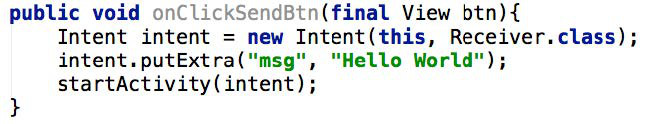
\includegraphics[width=\textwidth]{fig/send-explizit-intent}
		\caption{Expliziter Intent senden}
		\label{fig:send-explizit-intent}
	\end{subfigure}
	~
	\begin{subfigure}[b]{0.48\textwidth}
		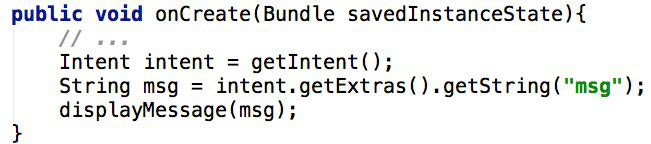
\includegraphics[width=\textwidth]{fig/receive-explizit-intent}
		\caption{Expliziter Intent empfangen}
		\label{fig:receive-explizit-intent}
	\end{subfigure}
	~
	\begin{subfigure}[b]{0.48\textwidth}
		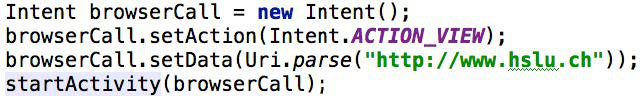
\includegraphics[width=\textwidth]{fig/send-implizit-intent}
		\caption{Impliziter Intent senden}
		\label{fig:send-implizit-intent}
	\end{subfigure}
	\caption{Intents aufrufen}
\end{figure}
Eine Activity kann auf Rückgabewerte einer anderen Activity (= Sub-Activity) warten. Nachfolgend ist dieser Ablauf beschrieben:
\begin{enumerate}
	\item Aufruf der SubActivity mit \texttt{startActivityForResult(intent, requestId)}
	\item SubActivity setzt am Ende Resultat mit \texttt{setResult(resultCode, intent)}
	\item SubActivity beendet sich mit \texttt{finish()}
	\item Nach Beendung der Sub-Activity wird \texttt{onActivityResult(requestId, resultCode, intent)} im Aufrufer aufgerufen
\end{enumerate}

\section{Lebenszyklus \& Zustände von Applikationen bzw. Activities}

Das System kann eine Applikation pausieren oder stoppen, wenn der Speicher knapp wird. Das System kontrolliert den Lebenszyklus von Applikationen (d.h. deren Komponenten) d.h. eine Applikation kann ihren Lebenszyklus nicht kontrollieren und muss daher u.a. in der Lage sein, ihren Zustand zu speichern und wieder zu laden. 
Eine Activity kann folgende Zustände haben:
\begin{description}
	\item[Running:]	Die Activity ist im Vordergrund auf dem Bildschirm (zuoberst auf dem Activity-Stack	für die aktuelle Aufgabe)
	\item[Paused] Die Activity hat den Fokus verloren, ist aber	immer noch sichtbar für den Benutzer
	\item[Stopped] Die Activity ist komplett verdeckt von einer	andern Activity. Der Zustand der Activity bleibt jedoch erhalten
\end{description}
Während den Zustandswechseln können folgende Callback-Methoden aufgerufen werden:
\begin{itemize}
	\item \texttt{onCreate()}
	\item \texttt{onStart()}
	\item \texttt{onResume()}	
	\item \texttt{onPause()}	
	\item \texttt{onStop()}	
	\item \texttt{onDestroy()}	
\end{itemize}
Es sollte immer die \texttt{super}-Methode überschrieben werden sonst gibt es eine Exception.

\section{Android: ein Blick hinter die Kulissen}

\subsection{Android Stack}

Abbildung \ref{fig:android-stack} zeigt einen Überblick über den Android Stack. Die Blau eingefärbten Bereiche sind in Java und der grüne Bereich ist in C/C++ geschrieben.

\begin{figure}
\centering
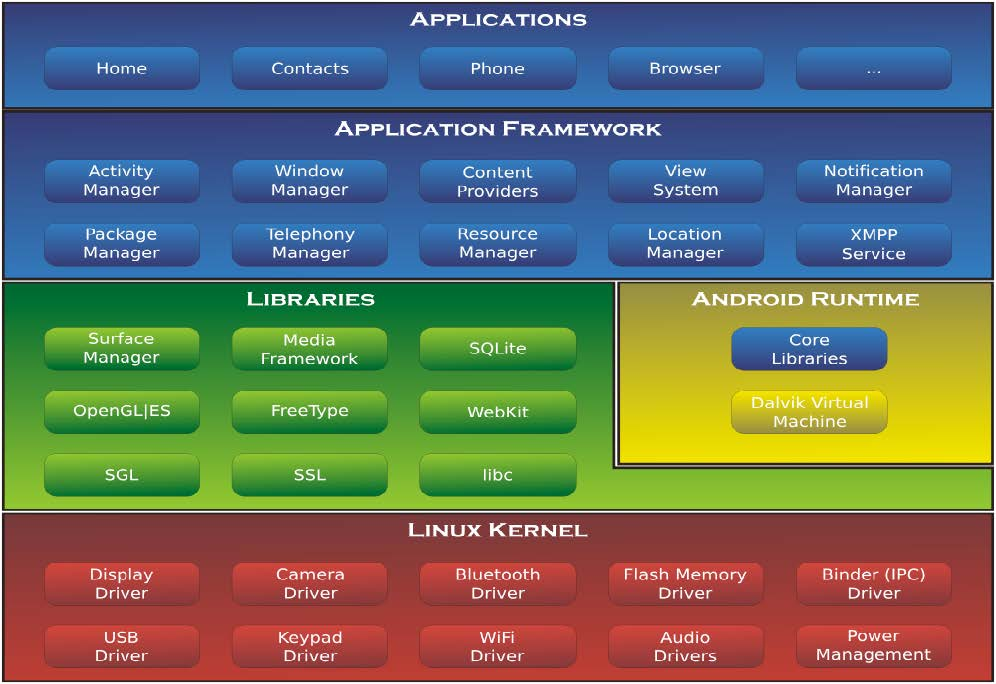
\includegraphics[width=0.7\linewidth]{fig/android-stack}
\caption{}
\label{fig:android-stack}
\end{figure}

Vor Android 5 war die Dalvik Virtual Machine die VM auf welcher die Java Programme ausgeführt wurden. Die DVM verwendet einen JIT (just-in-time) Compiler (Optimierungen zur Laufzeit) und ist optimiert für Systeme, welche beschränkt sind in Bezug auf Speicher und Prozessorgeschwindigkeit. Die Core Libraries entsprechen grösstenteils Java 5 SE und basieren auf dem Apache Harmony Projekt (ehemalige Java Open Source Implementierung). Android verwendet cross-compiling um Java auf der Dalvik-VM auszuführen. Die Kompilierung läuft wie folgt ab:
\begin{enumerate}
	\item Entwicklung der Applikation in Java
	\item Transformierung von Java-Bytecode (*.class) nach Dalvik-Bytecode (*.dex = Dalvik EXecutable)
	\item Deployment
	\item Ausführung *.dex Klassen auf der Dalvik-VM
\end{enumerate}
Mit Android 5 wurde Dalvik komplett gestrichen. Neu kommt die Android-Runtime (ART) zum Einsatz. ART verwendet dasselbe .dex-Format wie für die Dalvik-VM (Rückwärtskompatibilität) und bietet ahead-of-time (AOT) Kompilierung (d.h. Optimierungen zur Installationszeit).

\subsection{Android Security Konzept}

Android verwendet das Sandbox-Konzept d.h. jede laufende Android-Anwendung hat eigenen Prozess, Benutzer, DVM, Heap und Dateisystembereich. Zudem wird das Berechtigungssystem von Linux verwendet. Zudem werden Anwendungen zum Schutz gegen Code-Manipulationen signiert. Durch die im Manifest definierten Berechtigungen kann die Sandbox kontrolliert geöffnet werden.